\documentclass[12pt,a4paper]{article}
\usepackage[utf8]{inputenc} 
\usepackage[ngerman]{babel}
\usepackage[T1]{fontenc}
\usepackage{amsmath}
\usepackage{amsfonts}
\usepackage{amssymb}
\usepackage{graphicx}
\usepackage[left=2cm,right=2cm,top=2cm,bottom=2cm]{geometry}
\usepackage{physics}
\usepackage{float}
\usepackage{multirow}
\setlength{\parindent}{0pt}
\usepackage{enumitem}
\usepackage{xcolor}
\usepackage{cancel} 

\newcommand{\h}[2]{\color{#1} #2 \color{black} }

\newcommand{\equalInM}[1]{\h{blue}{#1}} % umfasst mehr; inkl. Vorzeichen gleich über Sym-Anti und Anti-Sym und über die versch. Tableaus dieser Kategorie
\newcommand{\equalInTableau}[1]{\h{magenta}{#1}} % Vorzeichen vertauscht zw. den versch. Tableaus, aber Vorzeichen gleich bzgl. Anti-Sym zu Sym-Anti-Tausch
\newcommand{\equalAntiSym}[1]{\h{brown}{#1}} % zwar nicht in allen Tableaus einer M Sorte, aber gleich (inkl. Vorzeichen) bzgl. der Anti-Sym und der Sym-Anti Rechnung



\usepackage{soul}   % Für das Hervorheben von Text


\setcounter{secnumdepth}{4} % Nummerierung bis zur 4. Ebene erlauben

\usepackage{titlesec}
\usepackage{hyperref} % Für klickbare Links im Inhaltsverzeichnis

% Anpassung der \paragraph{}-Überschrift
\titleclass{\paragraph}{straight}
\titleformat{\paragraph}[runin]{\normalfont\normalsize\bfseries}{\theparagraph}{1em}{}
\titlespacing*{\paragraph} {0pt}{3.25ex plus 1ex minus .2ex}{1.5ex plus .2ex}


\begin{document}

\title{analytische Betrachtung}

\tableofcontents
\newpage


\section{Spinfunktionen für $n_{el} = 4$}

\subsection{Quantenzahlen und Abkürzung als Ket}
 $n_{el} = 4$ d.h. $S = \{ 0, 1, 2\}$ und 
\begin{itemize}
\item $M_S = \{0\}$ für $S = 0$ bzw. $2S+1 = 1$
\item $M_S = \{-1, 0, 1\}$ für $S = 1$ bzw. $2S+1 = 3$
\item $M_S = \{-2, -1, 0, 1, 2\}$ für $S = 2$ bzw. $2S+1=5$
\end{itemize}


d.h. mögliche Fälle für $\ket{ S \; M_S }$ lauten: 
\begin{itemize}
\item $\ket{ 0\quad 0}$
\item $\ket{ 1 \quad 1}$
\item $\ket{ 1 \quad 0}$
\item $\ket{ 1 \quad -1}$
\item $\ket{ 2 \quad 2}$
\item $\ket{ 2 \quad 1}$
\item $\ket{ 2 \quad 0}$
\item $\ket{ 2 \quad -1}$
\item $\ket{ 2 \quad -2}$
\end{itemize}



Der Fall $\uparrow\uparrow\uparrow\uparrow$ muss symmetrisch sein und kann nur im Fall $S = 2$ vorkommen. D.h. $S=2$ gehört zum Tableau $\left[ 4\right]$, das nur Kästchen nur symmetrisch (= in 1 Reihe) kombiniert. Analog weitergegangen folgt: $\left[ 31\right]$ gehört zu $S = 1$ und $\left[ 2 ^2 \right]$ gehört zu $S = 0$. 

\begin{table}[H]
\centering
\begin{tabular}{|c|c|c|}
\hline
 $\left[ 4\right]$ & $\left[ 3\,1\right]$ & $\left[ 2^2\right]$ \\
\hline & & \\
 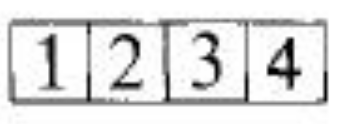
\includegraphics[scale=0.2]{build/young-4.png} & 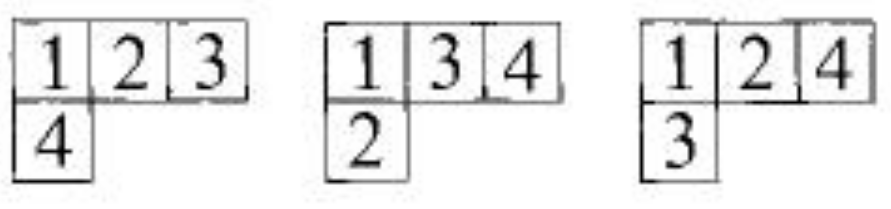
\includegraphics[scale=0.2]{build/young-31.png} & 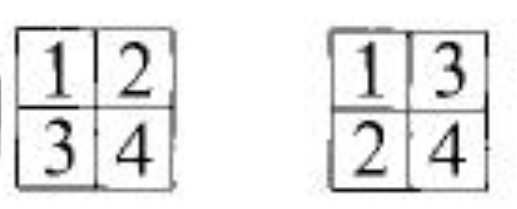
\includegraphics[scale=0.2]{build/young-2hoch2.png} \\
\hline
$\ket{ 2 \quad 2}$ &$\ket{ 1 \quad 1}$&$\ket{ 0\quad 0}$ \\
$\ket{ 2 \quad 1}$ &$\ket{ 1 \quad 0}$& \\
$\ket{ 2 \quad 0}$ &$\ket{ 1 \quad -1}$  & \\
$\ket{ 2 \quad -1}$ & & \\
$\ket{ 2 \quad -2}$ & & \\
\hline
\end{tabular}
\end{table}

\subsection{Funktionen}
Funktionen konstruieren anhand der $M_S$-Werte und daraus folgender mögl. $m_s$ Kombinationen. Vorzeichen anhand des Young-Tableau: \\


\begin{itemize}
\item $\left[ 4\right]$ :
\begin{itemize}
\item 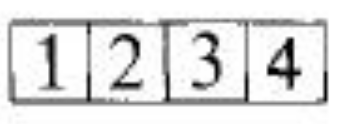
\includegraphics[scale=0.2]{build/young-4.png} : 
\begin{itemize}[label=$\ast$]
\item $\ket{2\quad2} = \left( \alpha \alpha \alpha\alpha\right)$ 
\item $\ket{2 \quad 1} = \frac{1}{\sqrt{4}} \left[
\left( \alpha\alpha\alpha\beta\right) + \left(\alpha \alpha\beta \alpha \right) 
+ \left(\alpha\beta\alpha \alpha\right) + \left( \beta\alpha \alpha\alpha\right) 
 \right]$ 
 \item  $\ket{2\quad 0} =\frac{1}{\sqrt{6}} \left[ 
\left(\alpha \alpha \beta \beta \right) + \left( \beta \alpha\beta \alpha \right) +
\left(\alpha\beta\alpha\beta \right) + \left(\beta \beta \alpha\alpha \right) +
\left( \alpha\beta\beta \alpha\right) + \left( \beta \alpha\alpha\beta\right) 
 \right]$ 
 \item  $\ket{2\quad -1} = \frac{1}{\sqrt{4}}  \left[ 
\left( \alpha\beta\beta\beta\right) + \left( \beta\alpha\beta\beta \right)  + 
\left( \beta\beta\alpha\beta \right) + \left( \beta \beta \beta \alpha\right) 
 \right]$
 \item $\ket{2\quad -2} = \left( \beta \beta \beta \beta \right) $
\end{itemize}
\end{itemize}
\item  $\left[ 3\quad 1\right]$ :
\begin{itemize}
\item  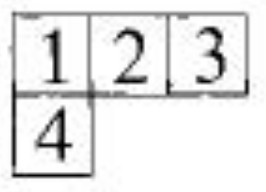
\includegraphics[scale=0.2]{build/young-31-123.png} : 
\begin{itemize}
\item  $\ket{1\quad 1} = \frac{1}{\sqrt{2}}  \left[ 
\left( \alpha\alpha\alpha \beta\right) - \left(  \beta \alpha\alpha\alpha\right) 
 \right]$
 \item  $\ket{1\quad 0} = \frac{1}{\sqrt{4}}  \left[ 
\left( \alpha\alpha\beta\beta \right) - \left( \beta \alpha\beta\alpha \right) +
\left( \alpha\beta \alpha\beta \right) - \left( \beta \beta \alpha\alpha\right) 
 \right]$
 \item  $\ket{1\quad -1} = \frac{1}{\sqrt{2}}  \left[ 
\left( \alpha\beta\beta\beta \right) - \left( \beta\beta\beta\alpha \right) 
 \right]$
\end{itemize}
\item 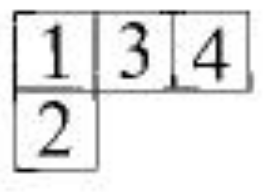
\includegraphics[scale=0.2]{build/young-31-134.png}: 
\begin{itemize}
\item $\ket{1\quad 1} = \frac{1}{\sqrt{2}}  \left[ 
\left( \alpha \beta \alpha\alpha \right) - \left( \beta \alpha\alpha\alpha\right) 
 \right]$
\item  $\ket{1\quad 0} = \frac{1}{\sqrt{4}}  \left[ 
\left( \alpha\beta\alpha\beta\right) - \left(\beta\alpha\beta\alpha \right) +
\left( \alpha\beta\beta\alpha \right) - \left( \beta \alpha\alpha\beta \right) 
 \right]$ 
\item  $\ket{1\quad -1} = \frac{1}{\sqrt{2}}  \left[ 
\left( \alpha\beta\beta\beta\right) - \left( \beta\alpha\beta\beta\right) 
 \right]$
\end{itemize}
\item 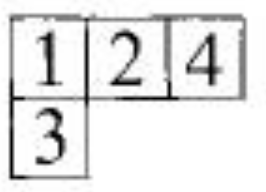
\includegraphics[scale=0.2]{build/young-31-124.png}: 
\begin{itemize}
\item $\ket{1\quad 1} = \frac{1}{\sqrt{2}}  \left[ 
\left( \alpha\alpha\beta\alpha \right) - \left( \beta\alpha\alpha\alpha\right) 
 \right]$
\item  $\ket{1\quad 0} = \frac{1}{\sqrt{4}}  \left[ 
\left( \alpha\alpha\beta\beta \right) - \left( \beta\alpha\alpha\beta\right) -
\left( \beta\beta\alpha\alpha  \right) + \left( \alpha\beta\beta\alpha \right)
 \right]$ 
\item  $\ket{1\quad -1} = \frac{1}{\sqrt{2}}  \left[ 
\left( \alpha\beta\beta\beta \right) - \left( \beta\beta\alpha\beta \right) 
 \right]$
\end{itemize}
\end{itemize}
\item $\left[ 2 ^2 \right]$ : 
\begin{itemize}
\item 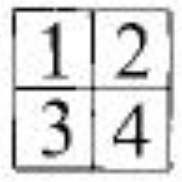
\includegraphics[scale=0.2]{build/young-2hoch2-12.png}
\begin{itemize}
\item  $\ket{0\quad 0} = \frac{1}{\sqrt{4}}  \left[ 
\left(\alpha\alpha\beta\beta \right) + \left( \beta\beta\alpha\alpha \right) -
\left( \alpha\beta \beta\alpha\right) - \left( \beta\alpha\alpha\beta\right)
 \right]$
\end{itemize}
\item 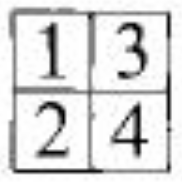
\includegraphics[scale=0.2]{build/young-2hoch2-13.png}
\begin{itemize}
\item  $\ket{0\quad 0} = \frac{1}{\sqrt{4}}  \left[ 
\left( \alpha\beta \alpha\beta\right) + \left( \beta\alpha\beta\alpha\right) 
 - \left( \alpha\beta\beta \alpha\right)  - \left( \beta\alpha\alpha\beta\right) 
 \right]$
\end{itemize}
\end{itemize}
\end{itemize}

\newpage
\subsection{Herleitung Spinfunktionen}
Vorfaktoren entsprechen nicht dem Normierungsfaktor, werden nur z.T. zur Nachvollziehbarkeit hier mitgeschrieben; grün hinterlegt = $\hat{A}\hat{S}$ und $\hat{S}\hat{A}$. identisch, bold = Unterschiedssummanden zw. $\hat{A}\hat{S}$ und $\hat{S}\hat{A}$. \\

\vspace{3cm}
\begin{table}[H]
\begin{tabular}{|p{2cm}|p{7cm}|p{7cm}|}
  \hline 
 & \multicolumn{2}{c|}{ 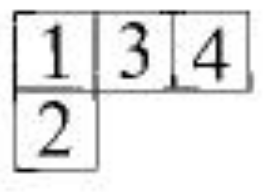
\includegraphics[scale=0.2]{build/young-31-134.png} } \\
  \hline 
& $\hat{A}\hat{S}$ & $\hat{S}\hat{A}$ \\ \hline 
$M_S = 0$ $\leftrightarrow$ $1=3=4=\alpha$, $ 2=\beta$ &    
\parbox[t][2em]{7cm}{ 
$ \hat{A}\left( \alpha\alpha\alpha \right) \beta$ \\
\colorbox{green}{ $
= \alpha\beta\alpha\alpha - \beta\alpha\alpha\alpha 
$}
   }
 &
\parbox[t][2em]{7cm}{ 
$ \hat{S}\left(\alpha\beta - \beta\alpha\right) \alpha\alpha$ \\
\colorbox{green}{ $= 6\;\alpha\beta\alpha\alpha - 6\;\beta\alpha\alpha\alpha $}
} 
  \\ \hline
 $M_S = 1$ $\leftrightarrow$ $1=3=\alpha$, $2=4=\beta$ & 
  \parbox[t][4em]{7cm}{ 
  $ \hat{A}\left(\alpha\alpha\beta + \beta\alpha\alpha + \alpha\beta\alpha \right)\beta$\\
  $
= \alpha\beta\alpha\beta - \beta\alpha\alpha\beta \boldsymbol{+ \beta\beta\alpha\alpha} - \beta\alpha\beta\alpha + \alpha\beta\beta\alpha \boldsymbol{- \alpha\alpha\beta\beta}$\\
  } & 
 \parbox[t][9em]{7cm}{ 
 $\hat{S} \left( \alpha\beta - \beta\alpha\right) \alpha\beta$\\
 $= \alpha\beta\alpha\beta + \alpha\beta\alpha\beta + \alpha\beta\beta\alpha + \beta\beta\alpha\alpha + \alpha\beta\beta\alpha + \beta\beta\alpha\alpha$\\$
-\beta\alpha\alpha\beta - \beta\alpha\alpha\beta - \beta\alpha\beta\alpha - \beta\beta\alpha\alpha - \beta\alpha\beta\alpha - \beta\beta\alpha\alpha$ \\
$ = 2\;\alpha\beta\alpha\beta + 2\;\alpha\beta\beta\alpha $ \\
$-2 \;\beta\alpha\alpha\beta - 2\;\beta\alpha\beta\alpha$
 }
  \\ \hline 
  $M_S = -1$ $\leftrightarrow$ $1=\alpha$, $2=3=4=\beta$ & 
  \parbox[t][2em]{7cm}{
  $\hat{A}\left( \alpha\beta\beta + \beta\alpha\beta + \beta\beta\alpha \right) \beta$\\
  $
 = \alpha\beta\beta\beta - \beta\alpha\beta\beta + \beta\beta\alpha\beta - \beta\alpha\beta\beta + \beta\beta\beta\alpha - \beta\alpha\beta\beta$\\
$= \alpha\beta\beta\beta - 3 \beta\alpha\beta\beta +  \beta\beta\alpha\beta + \beta\beta\beta\alpha$
  }
   & \parbox[t][10em]{7cm}{
   $\hat{S} \left(\alpha\beta - \beta\alpha \right) \beta\beta$\\
   $= \alpha\beta\beta\beta + \beta\beta\alpha\beta + \alpha\beta\beta\beta + \beta\beta\beta\alpha + \beta\beta\beta\alpha + \beta\beta\alpha\beta$\\$
-\beta\alpha\beta\beta - \beta\beta\alpha\beta - \beta\alpha\beta\beta - \beta\beta\beta\alpha - \beta\beta\beta\alpha - \beta\beta\alpha\beta
$ \\
$=2\;\alpha\beta\beta\beta - 2\;\beta\alpha\beta\beta $
}
  \\ \hline 
\end{tabular}
\end{table}


\vspace{3cm}
\begin{table}[H]
\begin{tabular}{|p{2cm}|p{7cm}|p{7cm}|}
  \hline 
 & \multicolumn{2}{c|}{ 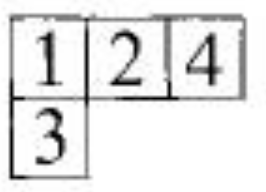
\includegraphics[scale=0.2]{build/young-31-124.png} } \\
  \hline 
& $\hat{A}\hat{S}$ & $\hat{S}\hat{A}$ \\ \hline 
$M_S = 0$ $\leftrightarrow$ $1=2=4=\alpha$, $ 3=\beta$ &    
\parbox[t][6em]{7cm}{ 
$\hat{A}\left(\alpha\alpha\alpha \right) \beta$\\
\colorbox{green}{ $= \alpha\alpha\beta\alpha - \beta\alpha\alpha\alpha$}
   }
 &
\parbox[t][2em]{7cm}{ 
$\hat{S} \left(\alpha\beta - \beta\alpha\right) \alpha\alpha$\\
\colorbox{green}{ $
= 6\;\alpha\alpha\beta\alpha -6\;\beta\alpha\alpha\alpha $}
} 
  \\ \hline
 $M_S = 1$ $\leftrightarrow$ $1=2=\alpha$, $3=4=\beta$ & 
  \parbox[t][4em]{7cm}{ 
  $\hat{A}  \left(\alpha\alpha\beta + \beta\alpha\alpha + \alpha\beta\alpha \right) \beta$\\
  $= \alpha\alpha\beta\beta - \beta\alpha\alpha\beta  \boldsymbol{+ \beta\alpha\beta\alpha} - \beta\beta\alpha\alpha + \alpha\beta\beta\alpha \boldsymbol{- \alpha\beta\alpha\beta}$\\
  } & 
 \parbox[t][9em]{7cm}{ 
 $\hat{S} \left(\alpha\beta - \beta\alpha\right) \alpha\beta$\\
 $= \alpha\alpha\beta\beta + \alpha\alpha\beta\beta + \alpha\beta\beta\alpha + \beta\alpha\beta\alpha + \alpha\beta\beta\alpha + \beta\alpha\beta\alpha$\\$
-\beta\alpha\alpha\beta - \beta\alpha\alpha\beta - \beta\beta\alpha\alpha - \beta\alpha\beta\alpha - \beta\alpha\beta\alpha - \beta\beta\alpha\alpha$
\\ $= 2\; \alpha\alpha\beta\beta + 2\; \alpha\beta\beta\alpha 
- 2\;\beta\alpha\alpha\beta - 2\;\beta\beta\alpha\alpha
$
 }
  \\ \hline 
  $M_S = -1$ $\leftrightarrow$ $1=\alpha$, $2=3=4=\beta$ & 
  \parbox[t][2em]{7cm}{
  $\hat{A}\left( \alpha\beta\beta + \beta\alpha\beta + \beta\beta\alpha \right) \beta$ \\$
= \alpha\beta\beta\beta - \beta\beta\alpha\beta + \beta\alpha\beta\beta - \beta\beta\alpha\beta + \beta\beta\beta\alpha - \beta\beta\alpha\beta$\\
$ = \alpha\beta\beta\beta - 3 \beta\beta\alpha\beta \boldsymbol{+ \beta\alpha\beta\beta + \beta\beta\beta\alpha} $
  }
   & \parbox[t][10em]{7cm}{
   $\hat{S} \left(\alpha\beta - \beta\alpha\right) \beta\beta$\\
   $= \alpha\beta\beta\beta + \beta\alpha\beta\beta + \alpha\beta\beta\beta + \beta\beta\beta\alpha + \beta\beta\beta\alpha + \beta\alpha\beta\beta$\\$
-\beta\beta\alpha\beta - \beta\alpha\beta\beta - \beta\beta\alpha\beta - \beta\beta\beta\alpha - \beta\alpha\beta\beta - \beta\beta\beta\alpha$ \\
$=2 \;\alpha\beta\beta\beta  - 2\; \beta\beta\alpha\beta$
}
  \\ \hline 
\end{tabular}
\end{table}


\vspace{3cm}
\begin{table}[H]
\begin{tabular}{|p{2cm}|p{7cm}|p{7cm}|}
  \hline 
 & \multicolumn{2}{c|}{ 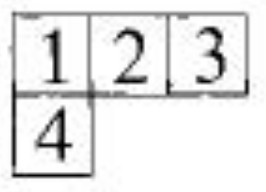
\includegraphics[scale=0.2]{build/young-31-123.png} } \\
  \hline 
& $\hat{A}\hat{S}$ & $\hat{S}\hat{A}$ \\ \hline
$M_S = 0$ $\leftrightarrow$ $1=2=3=\alpha$, $ 4=\beta$ &    
\parbox[t][2em]{7cm}{ 
  $ A\left( \alpha\alpha\alpha \right) \beta $ \\
   $ = \alpha\alpha\alpha\beta -  \beta\alpha\alpha\alpha$
   }
 &
\parbox[t][2em]{7cm}{ 
$ \hat{S}\left( \alpha\beta - \beta \alpha\right) \alpha\alpha$  \\
\colorbox{green}{$= 6 \; \alpha\alpha\alpha\beta $
$ - 6\; \beta\alpha\alpha\alpha$}
} 
  \\ \hline
 $M_S = 1$ $\leftrightarrow$ $1=2=\alpha$, $3=4=\beta$ & 
  \parbox[t][4em]{7cm}{ 
  $\hat{A}\left( \alpha\alpha\beta + \alpha\beta\alpha+ \beta\alpha\alpha \right)\beta$ \\
  $= \alpha\alpha\beta\beta - \beta\alpha\beta\alpha+\alpha\beta\alpha\beta
  - \beta\beta\alpha\alpha $\\$ \cancel{+ \beta \alpha\alpha\beta}
  \cancel{ - \beta\alpha\alpha\beta}
$  } & 
 \parbox[t][9em]{7cm}{ 
 $\hat{S} \left(\alpha\beta - \beta \alpha\right) \alpha\alpha$ \\
 $ = \alpha\alpha\beta\beta + \alpha\alpha\beta\beta + \alpha\beta\alpha\beta
 + \beta\alpha\alpha\beta + \alpha\beta \alpha\beta + \beta\alpha\alpha\beta$ \\
 $ - \beta\alpha\beta\alpha - \alpha\beta\beta\alpha - \beta\beta \alpha\alpha
 -\beta\alpha\beta\alpha - \alpha\beta\beta\alpha - \beta\beta\alpha\alpha$ \\
 $= 2\; \alpha\alpha\beta\beta - 2\;\alpha\beta\alpha\beta
 - 2\;\beta\alpha\beta\alpha  - 2 \;\alpha\beta\beta\alpha $ \\
$ \boldsymbol{+ 2\; \beta\alpha\alpha\beta - 2 \;\beta\beta\alpha\alpha}$
 }
  \\ \hline 
  $M_S = -1$ $\leftrightarrow$ $1=\alpha$, $2=3=4=\beta$ & 
  \parbox[t][2em]{7cm}{
  $\hat{A}\left(\alpha\beta\beta\right)\beta $ \\
  $ = \alpha\beta\beta\beta - \beta\beta\beta\alpha 
   $
  }
   & \parbox[t][10em]{7cm}{
   $ \hat{S}\left( \alpha\beta - \beta \alpha\right) \beta\beta$ \\
   $ = \alpha\beta\beta\beta + \beta\alpha\beta\beta+  \beta\beta\alpha\beta
   + \alpha\beta\beta\beta + \beta\beta\alpha\beta + \beta\alpha\beta\beta$ \\
   $ - \beta\beta\beta\alpha - \beta\alpha\beta\beta - \beta\beta\beta\alpha 
   - \beta\beta\alpha\beta - \beta\alpha\beta\beta - \beta\beta\alpha\beta 
    $  \\
\colorbox{green}{  $ = 2\;\alpha\beta\beta\beta - 2\;\beta\beta\beta\alpha $} 
   \\ (2. Teil: Festhalten des Index 4, der nun an 1. Stelle steht!)
    }
  \\ \hline 
\end{tabular}
\end{table}

\begin{table}[H]
\begin{tabular}{|p{2cm}|p{7cm}|p{7cm}|}
  \hline 
 & \multicolumn{2}{c|}{ 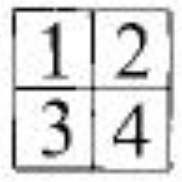
\includegraphics[scale=0.2]{build/young-2hoch2-12.png} } \\
  \hline 
& $\hat{A}\hat{S}$ & $\hat{S}\hat{A}$ \\ \hline
$M_S = 0$ $\leftrightarrow$ $1=2=\alpha$, $ 3=4=\beta$ & 
\parbox[t][11em]{7cm}{
$\hat{A} \left( \alpha\alpha \right) \left(\beta\beta\right) $ \\
$
\alpha\alpha\beta\beta - \beta\alpha\alpha\beta - \alpha\beta\beta\alpha + \beta\beta\alpha\alpha $\\
$+ \alpha\alpha\beta\beta - \alpha\beta\alpha\beta - \beta\alpha \beta \alpha 
+ \beta\beta\alpha\alpha $ \\
 $ = 2\;\alpha\alpha\beta\beta 
 - \beta\alpha\alpha\beta - \alpha\beta\beta\alpha
  \boldsymbol{- \alpha\beta\alpha\beta - \beta\alpha\beta\alpha}
 + 2\;\beta\beta\alpha\alpha  $ \\
 (wenn Wegfall von Termen nach S nicht beachtet wird, und nur 1234 ersetzt werden, ergibt sich eine Wiederholung aller Summanden = Dopplung)
} & 
\parbox[t][10em]{7cm}{
$\hat{S}\left( \alpha\beta -\beta\alpha\right)\left(\alpha\beta - \beta\alpha \right)$ \\
$ = \hat{S}\left( \alpha\beta -\beta\alpha\right)\alpha\beta - \hat{S} \left( \alpha\beta -\beta\alpha\right) \beta\alpha  $ \\
$= \alpha\alpha\beta\beta - \beta\alpha\alpha\beta - \alpha\beta\beta\alpha + \beta\beta\alpha\alpha + \alpha\alpha\beta\beta - \alpha\beta\alpha\beta - \beta\alpha\beta\alpha + \beta\beta\alpha\alpha +\alpha\alpha\beta\beta$ \\$
 - \beta\alpha\beta\alpha - \alpha\beta\alpha\beta + \beta\beta\alpha\alpha + \alpha\alpha\beta\beta - \alpha\beta\beta\alpha - \beta\alpha\alpha\beta + \beta\beta\alpha\alpha $ \\
$= 4\;\alpha\alpha\beta\beta 
- 4\;\beta\alpha\alpha\beta
- 4\; \alpha\beta\beta\alpha
- 4\; \beta\beta\alpha\alpha$
} \\ \hline
\end{tabular}
\end{table}


\begin{table}[H]
\begin{tabular}{|p{2cm}|p{7cm}|p{7cm}|}
  \hline 
 & \multicolumn{2}{c|}{ 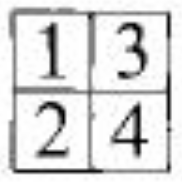
\includegraphics[scale=0.2]{build/young-2hoch2-13.png} } \\
  \hline 
& $\hat{A}\hat{S}$ & $\hat{S}\hat{A}$ \\ \hline
$M_S = 0$ $\leftrightarrow$ $1=2=\alpha$, $ 3=4=\beta$ & 
\parbox[t][10em]{7cm}{
$\hat{A}\left(\alpha\beta + \beta\alpha\right)\left(\alpha\beta + \beta\alpha\right) $\\
$= \hat{A}\left(\alpha\beta + \beta\alpha\right)\alpha\beta - \hat{A}\left(\alpha\beta + \beta\alpha\right)\beta\alpha$\\
$= \alpha\alpha\beta\beta - \alpha\alpha\beta\beta - \alpha\alpha\beta\beta + \alpha\alpha\beta\beta $\\
$+ \beta\alpha\alpha\beta - \beta\alpha\alpha\beta - \beta\alpha\alpha\beta + \beta\alpha\alpha\beta$\\
$-\alpha\beta\beta\alpha + \alpha\beta\beta\alpha + \alpha\beta\beta\alpha - \alpha\beta\beta\alpha $\\$
- \beta\beta\alpha\alpha + \beta\beta\alpha\alpha + \beta\beta\alpha\alpha - \beta\beta\alpha\alpha
$\\
$= 0 $
} & 
\parbox[t][10em]{7cm}{
$\hat{S}\left(\alpha\alpha - \alpha\alpha\right)\left(\beta\beta - \beta\beta\right) $\\
$= \hat{S}\left(\alpha\alpha - \alpha\alpha\right)\beta\beta - \hat{S}\left(\alpha\alpha - \alpha\alpha\right)\beta\beta$\\
$= \alpha\alpha\beta\beta + \beta\alpha\alpha\beta + \alpha\beta\beta\alpha + \beta\beta\alpha\alpha $\\$- \alpha\alpha\beta\beta - \alpha\beta\alpha\beta - \beta\alpha\beta\alpha - \beta\beta\alpha\alpha$ \\
$= \beta\alpha\alpha\beta+ \alpha\beta\beta\alpha 
- \alpha\beta\alpha\beta- \beta\alpha\beta\alpha $
 
} \\ \hline
\end{tabular}
\end{table}


\subsection{Überlappungsintegrale}
\begin{enumerate}
\item Überlappungsintegrale zw. versch. Tableaus sind orthogonal
\item Überlappungsintegrale = 0 zwischen den versch. Kets eines Tableaus (da $M_S$ und damit die Anzahl der Spins ja verschieden, kann nie gleiche Folge vorkommen)
\item Überlappungsintegrale zw. versch. Tableaus eines Diagramms (= Form des Tableaus) können 0 oder 1/2 sein: 0 wenn $M_S$ versch., sonst 1/2
\end{enumerate}


 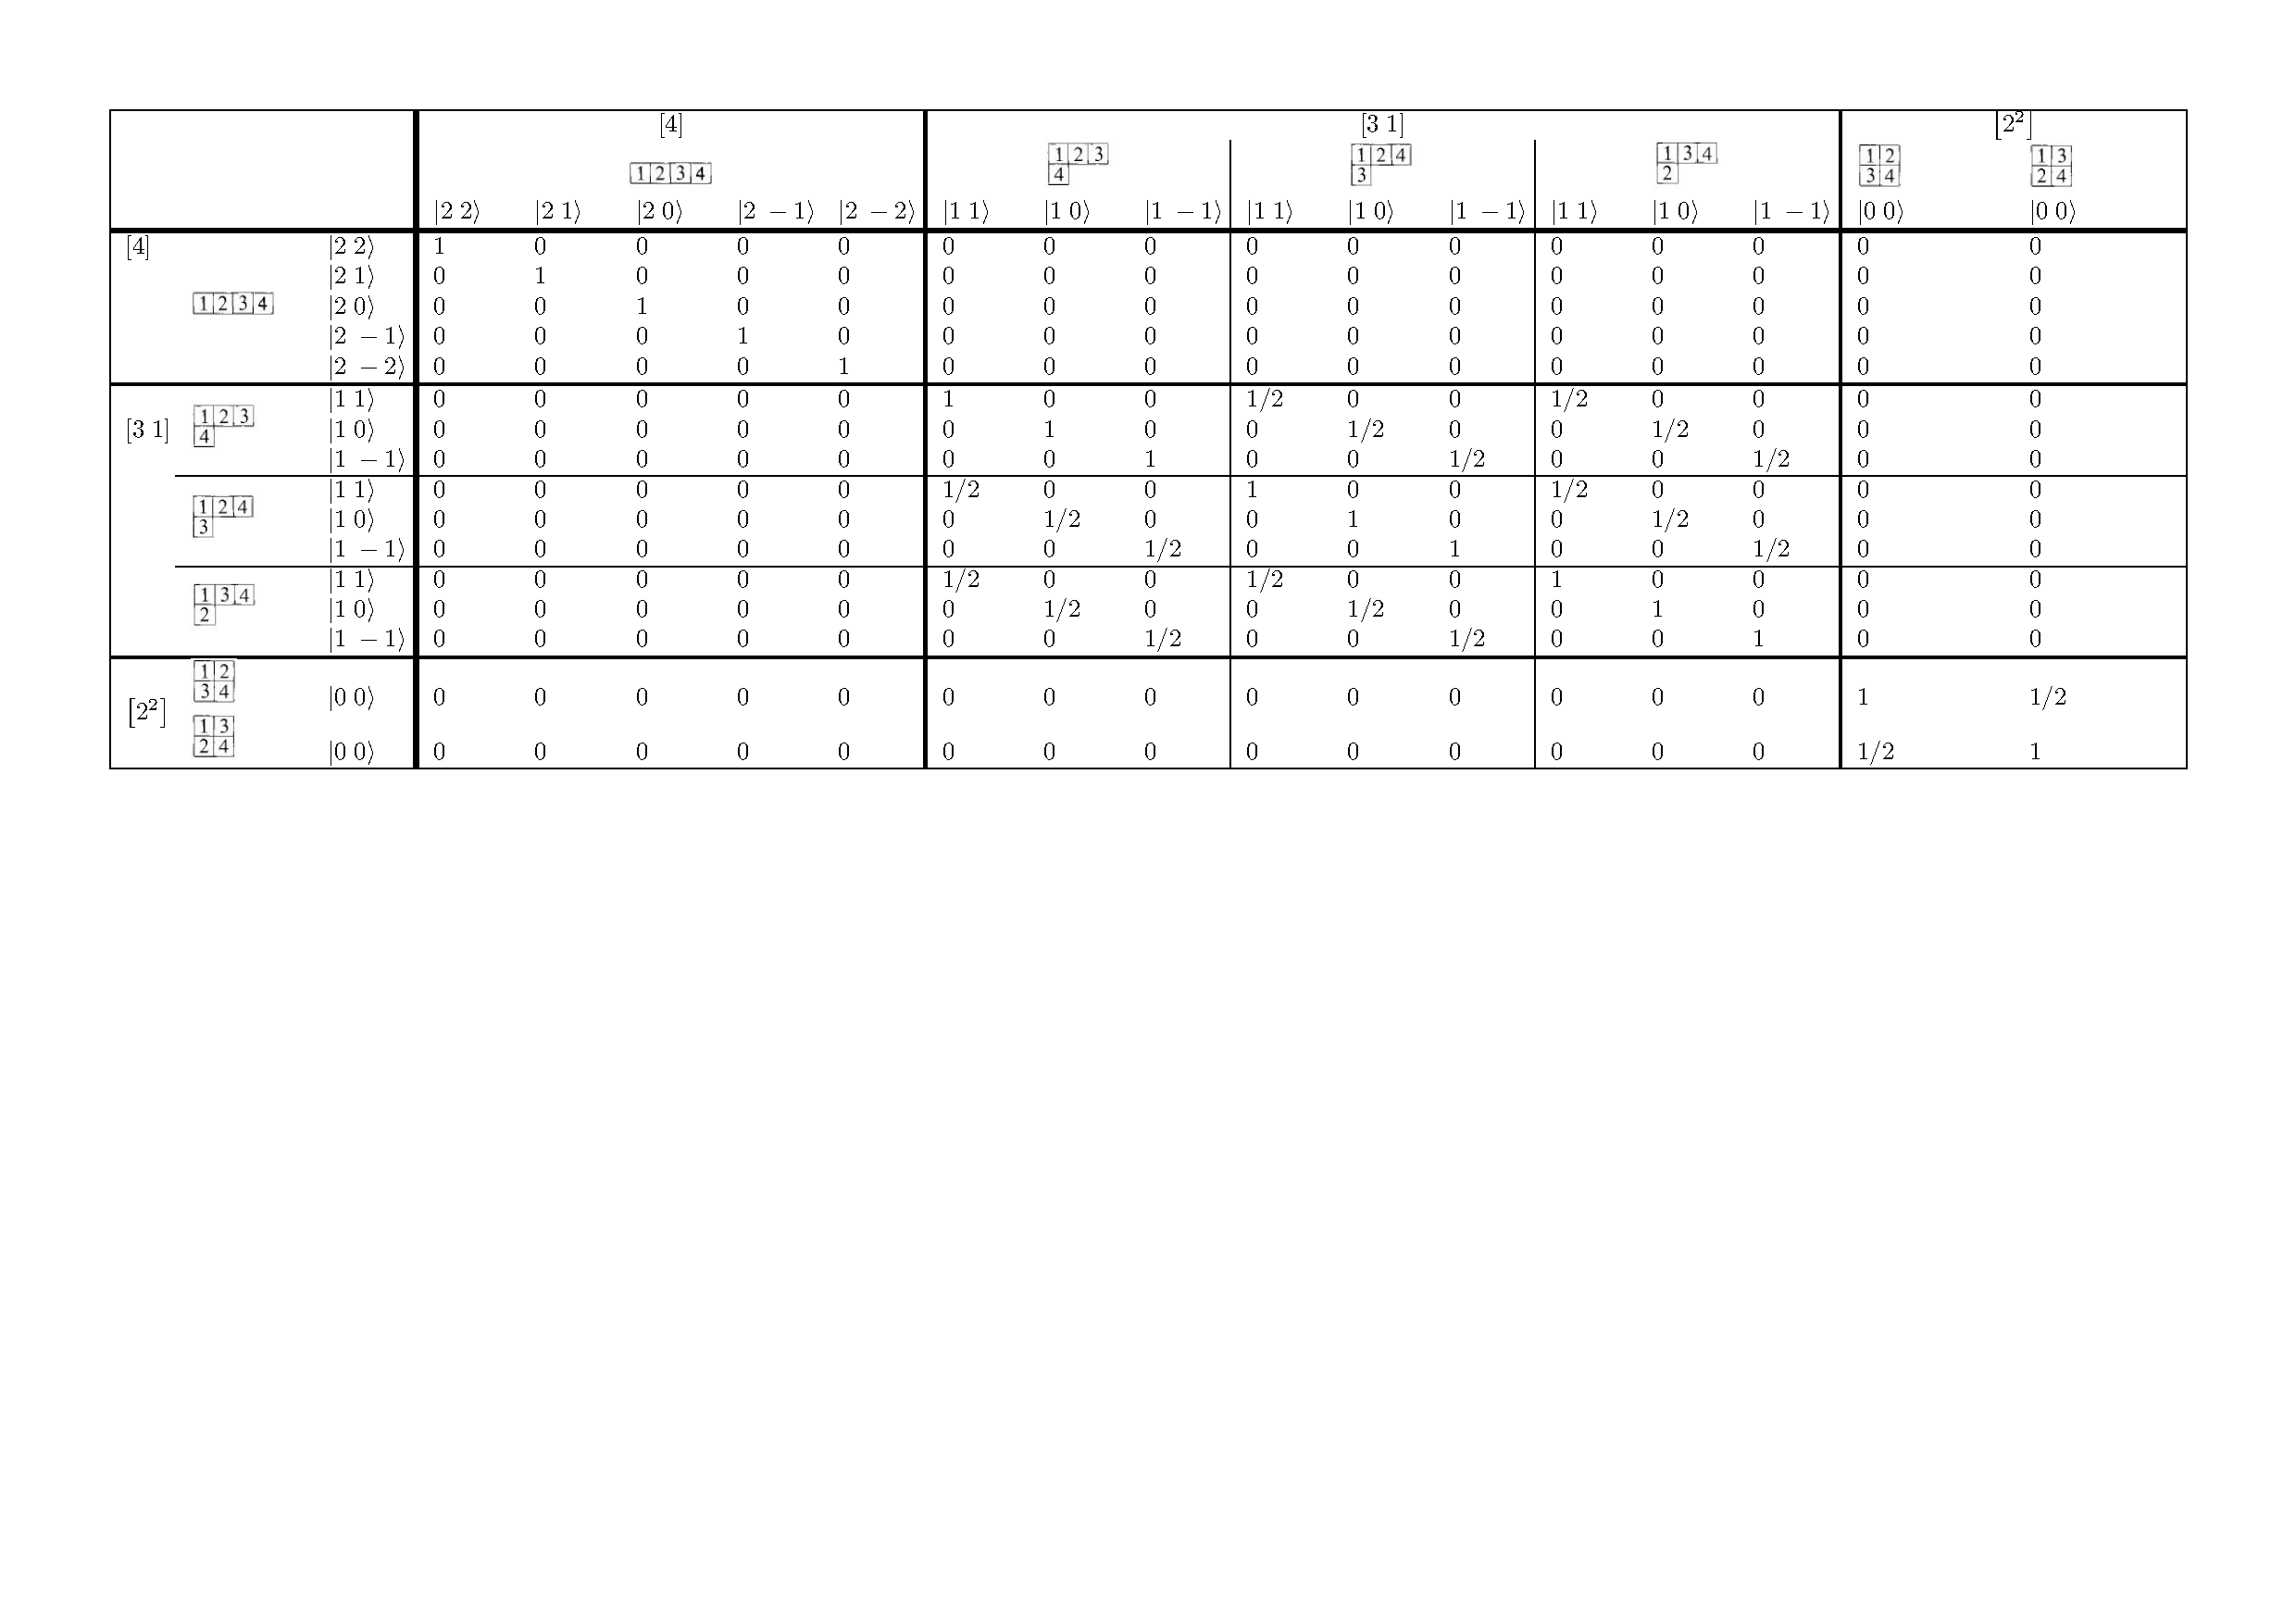
\includegraphics[scale=0.4]{build/Ueberlappung_Spin_cropped.pdf}




 \newpage
 \section{Raumfunktionen} 
 
 \subsection{Quantenzahlen und Abkürzung als Ket}
 
 4 Elektronen, von denen jeweils 2 im $e_{1g}$ und im $e_{2g}$ Orbital sind:
 $$ l_1 = 1,\quad l_2 = -1, \quad l_3 = 2, \quad l_4 = -2$$
 D.h. $L = {0, 2, 4}$ und 
 \begin{itemize}
 \item $M_L  = \{ \}$ für $L = 0$
 \item $M_L  = \{ -2, -1, 0, 1, 2 \}$ für $L = 2$
 \item $M_L  = \{ -4, -3, -2, -1, 0, 1, 2, 3, 4\}$ für $L = 4$
 \end{itemize}
 d.h. mögliche Fälle für $\ket{L \; M_L}$ lauten: 
 \begin{itemize}
 \item $\ket{ 0 \; 0}$ 
 \item $\ket{2 \quad 2}$, $\ket{2 \quad 1}$, $\ket{2 \quad 0}$, $\ket{2 \quad-1}$, $\ket{2 \quad -2}$
 \item $\ket{4\quad 4}$, $\ket{4\quad 3}$, $\ket{4\quad 2}$, $\ket{4\quad 1}$, $\ket{4\quad 0}$, $\ket{4\quad -1}$, $\ket{4\quad -2}$, $\ket{4\quad -3}$, $\ket{4\quad -4}$
 \end{itemize}
 
 adjungierte Young-Tableaus zu denen der Spinfunktionen: 
 \begin{table}[H]
\centering
 \begin{tabular}{|c|c|c|}
 \hline 
 $\left[1 ^4\right]$ & $\left[ 1 3\right]$ & $\left[ 2 ^2 \right]$ \\ \hline 
 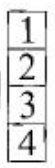
\includegraphics[scale=0.4]{build/young-1hoch4.png} & 
 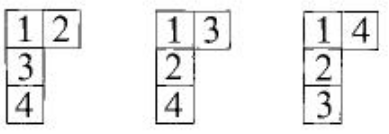
\includegraphics[scale=0.4]{build/young-21hoch2.png}
 & 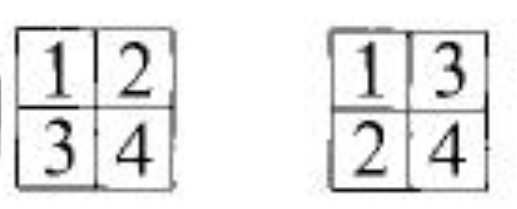
\includegraphics[scale=0.2]{build/young-2hoch2.png} \\ \hline 
 $\ket{4\quad 4}$ & $\ket{2\quad 2}$ & $\ket{0 \quad 0}$ \\
 $\ket{4\quad 3}$ & $\ket{2 \quad 1}$ & \\
 $\ket{4 \quad 2}$ & $\ket{2 \quad 0}$ & \\
 $\ket{4\quad 1}$ & $\ket{2 \quad -1}$ & \\
 $\ket{4\quad 0}$ & $\ket{2 \quad -2}$ & \\
 $\ket{4\quad -1}$ & & \\
 $\ket{4 \quad -2}$ & & \\
 $\ket{4 \quad -3}$ & & \\
 $\ket{4\quad -4}$ & & \\  \hline
 \end{tabular}
 \end{table}
 
 \newpage
\subsection{Funktionen}
\subsubsection{1. Antisymmetrisieren, 2. Symmetrisieren}
\begin{itemize}
\item $\left[ 1 ^4\right]$ 
\begin{itemize}
\item 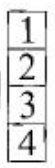
\includegraphics[scale=0.4]{build/young-1hoch4.png} :
\begin{itemize}
\item \equalInM{$
+1234-1243-1324+1342
+1423-1432 $\\
$-2134+2143 +2314-2341-2413+2431$\\
$+3124-3142-3214+3241 +3412-3421$\\
$-4123+4132 +4213-4231-4312+4321$ \\
$ = \begin{vmatrix}
1 & 1 & 1 & 1 \\
2 & 2 & 2 & 2 \\
3 & 3 & 3 & 3 \\
4 & 4 & 4 & 4 \\
\end{vmatrix}$}
\item Integrale: \\
$+ D + 1/6 \cdot (cd|dc) + 1/6 \cdot (bc|cb) - 1/6 \cdot (bd|db) - 1/6 \cdot (ab|ba) - 1/6 \cdot (ac|ca) - 1/6 \cdot (ad|da)$
\end{itemize}
\end{itemize}
\item $\left[ 2 1 ^2\right]$
\begin{itemize}
\item 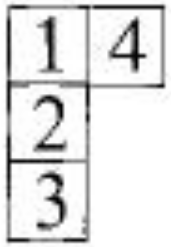
\includegraphics[scale=0.2]{build/young-21hoch2-14.png}
\begin{itemize}
\item $\hat{S} \left(
123 + 312 + 231 - 213 - 132 - 321
 \right) 4$ \\ 
 $= \equalInM{1234}  \equalInTableau{+ 4231} 
 \equalAntiSym{+ 3124 }+ 3421 
 \equalAntiSym{+ 2314 }+ 2341$\\
 $\equalInTableau{-2134} - 2431 
 \equalAntiSym{- 1324} \equalAntiSym{ - 4321}
  \equalInTableau{- 3214} - 3241$ \\
  $= \begin{vmatrix} 123\end{vmatrix} 4 $
  \\ bzw. $abcd + dbca + bcad + dcab + cabd + dabc$\\$
-bacd - dacb - acbd - dcba - cbad - dbac = \begin{vmatrix}
abc\end{vmatrix}d$
\item Integrale mit Vorfaktoren $\frac{1}{\sqrt{12} }$ werden zu: \\
$ + D + \frac{1}{3} \cdot (ad|da) - 1 \cdot (ab|ba) - 1 \cdot (bc|cb) - 1 \cdot (ac|ca) + \frac{1}{3} \cdot (bd|db) + \frac{1}{3} \cdot (cd|dc) $ 
\end{itemize}
\item 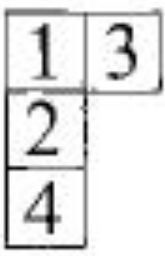
\includegraphics[scale=0.2]{build/young-21hoch2-13.png}
\begin{itemize}
\item $\hat{S} \left(
124 + 412 + 241 - 214 - 142 - 421
 \right) 3$ \\ 
 $ = \equalInM{1234}  \equalInTableau{+ 3214 }
 \equalAntiSym{+ 4132} + 4312 
 \equalAntiSym{+ 2431} + 2413 
 $\\
 $  \equalInTableau{- 2134 } - 2314 
 \equalAntiSym{- 1432} \equalAntiSym{ - 3412 }
 \equalInTableau{- 4231} - 4213$
 \\ bzw. $abcd + cbad + bdca + cdba + dacb + cadb$\\$
-bacd - cabd - adcb - cdab - dbca - cbda
$
\item Integrale mit Vorfaktoren $\frac{1}{\sqrt{12} }$ werden zu: \\
$ + D + \frac{1}{3}  \cdot (ac|ca) - 1 \cdot (ab|ba) - 1 \cdot (bd|db) - 1 \cdot (ad|da) + \frac{1}{3}  \cdot (bc|cb) + \frac{1}{3}  \cdot (cd|dc) 
 $
\end{itemize}
\item 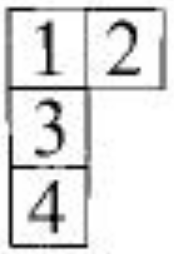
\includegraphics[scale=0.2]{build/young-21hoch2-12.png}
\begin{itemize}
\item $\hat{S} \left(
134 + 413 + 341 - 143 - 431 - 314
 \right) 2$ \\ 
 $= \equalInM{1234}  \equalInTableau{+ 2134 }
 \equalAntiSym{+4213} + 4123 
 \equalAntiSym{+ 3241} + 3142
 $\\
 $ \equalAntiSym{-1243} \equalAntiSym{ - 2143}
 \equalInTableau{- 4231} - 4132 
 \equalInTableau{- 3214} - 3124
 $ \\bzw. $abcd + bacd + cbda + bcda + dbac + bdac$\\$
-abdc - badc - dbca - bdca - cbad - bcad$
\item Integrale: 
$+ D + \frac{1}{3} \cdot (ab|ba) - 1 \cdot (cd|dc) - 1 \cdot (ad|da) - 1 \cdot (ac|ca) + \frac{1}{3} \cdot (bc|cb) + \frac{1}{3} \cdot (bd|db)$
\end{itemize}
\end{itemize}
\item $\left[ 2 ^2 \right]$ 
\begin{itemize}
\item 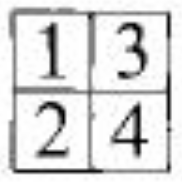
\includegraphics[scale=0.2]{build/young-2hoch2-13.png}
\begin{itemize}
\item $\hat{S} (12- 21) (34 - 43) = \left[ \hat{S} (12-21) 34 \right] - \left[ \hat{S} (12 - 21)43\right]$ \\ 
$ = \equalInM{1234} \equalInTableau{+ 3214} \equalInTableau{+ 1432} \equalInM{+ 3412 }
\equalInTableau{- 2134 } - 2314 - 4132 \equalInTableau{- 4312 } $\\
$\equalInTableau{- 1243 } - 3241 - 1423 \equalInTableau{- 3421 }
\equalInM{+ 2143} \equalInTableau{ + 2341 } \equalInTableau{+ 4123} + \equalInM{4321}$ \\
bzw. $abcd + cbad + adcb + cdab - bacd - cabd - bdca - cdba$\\$
-abdc - dbac - acdb - dcab + badc + dabc + bcda + dcba$
\item Integrale \\
$+ D + \frac{1}{2} \cdot (ac|ca) + \frac{1}{2} \cdot (bd|db) - 1 \cdot (ab|ba) - 1 \cdot (cd|dc) + \frac{1}{2} \cdot (bc|cb) + \frac{1}{2} \cdot (ad|da) $
\end{itemize}
\item 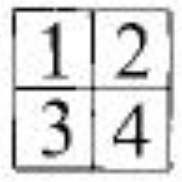
\includegraphics[scale=0.2]{build/young-2hoch2-12.png}
\begin{itemize}
\item $\hat{S} (13 -31) (24-42) = \left[ \hat{S} (13-31) 24 \right] - \left[ \hat{S} (13-31)42\right]$ \\ 
$= \equalInM{1234} \equalInTableau{+2134} \equalInTableau{+ 1243} \equalInM{+ 2143 }
\equalInTableau{- 3214 } - 3124 -4213 \equalInTableau{- 4123} $\\
$ \equalInTableau{-1432} - 2431 - 1342 \equalInTableau{- 2341}
\equalInM{+ 3412} \equalInTableau{+ 3421} \equalInTableau{+ 4312} \equalInM{+ 4321 }$ \\
bzw. $abcd + bacd + adcb + dbca + dacb + bdca$\\
$-cbad - bcad - cdab - dbac - bdac - dcab$
\item Integrale\\
$ + D + \frac{1}{2} \cdot (ab|ba) + 1 \cdot (bd|db) + \frac{1}{2} \cdot (ad|da) - 1 \cdot (ac|ca) + \frac{1}{2} \cdot (bc|cb) + \frac{1}{2} \cdot (cd|dc)$
\end{itemize}
\end{itemize}

\item  $\left[ 3\quad 1\right]$ :
\begin{itemize}
\item  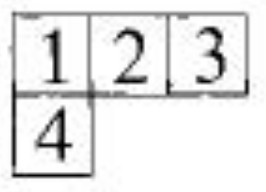
\includegraphics[scale=0.2]{build/young-31-123.png} : 
\begin{itemize}
 \item  $\hat{S} \left( 14 -41\right)23 $ \\
 $= 1234 + 2134 + 1324 + 3214 + 2314 + 3124 $ \\
 $- 4231 - 4132 - 4321 - 4213 - 4123 - 4312 $ 
\end{itemize}
\item 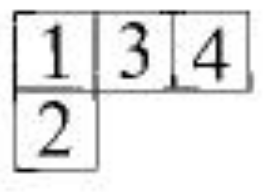
\includegraphics[scale=0.2]{build/young-31-134.png}: 
\begin{itemize}
\item  $ \hat{S} \left( 12-21\right)34$\\
  $= 1234 + 3214 + 1243 + 4231 + 3241 + 4213$  \\
  $ - 2134 - 2314 - 2143 - 2431 - 2341 - 2413$ 
\end{itemize}
\item 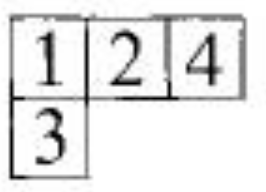
\includegraphics[scale=0.2]{build/young-31-124.png}: 
\begin{itemize}
\item $ \hat{S} \left(13 -31 \right)24$\\
  $= 1234 + 2134 + 1432 + 4231 + 2431 + 4132$  \\
  $ - 3214 - 3124 - 3412 - 3241 - 3142 - 3421$ 
\end{itemize}
\end{itemize}
\item $\left[ 4\right]$ :
\begin{itemize}
\item 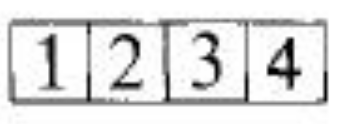
\includegraphics[scale=0.2]{build/young-4.png} : 
\begin{itemize}[label=$\ast$]
 \item \equalInM{$1234 + 1243 + 1324 + 1342 + 1423 + 1432  $\\
 $ + 2134 + 2143 + 2314 + 2341 + 2413+2431$ \\
 $ + 3124 + 3142 + 3214 + 3241 + 3412 + 3421 $\\
 $ + 4123 + 4132 + 4213 + 4231 + 4312 + 4321 $}
\end{itemize}
\end{itemize}
\end{itemize}








 \newpage
 \subsubsection{1. Symmetrisieren, 2. Antisymmetrisieren}
% = Georgs Variante 
\begin{itemize}
\item $\left[ 1 ^4\right]$ 
\begin{itemize}
\item 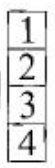
\includegraphics[scale=0.4]{build/young-1hoch4.png} :
\begin{itemize}
\item \equalInM{$
+1234-1243-1324+1342
+1423+1432 $\\
$-2134-2143 -2314-2341-2413+2431$\\
$+3124-3142+3214+3241 -3412-3421$\\
$-4123+4132 -4213-4231-4312-4321$ \\
$ = \begin{vmatrix}
1 & 1 & 1 & 1 \\
2 & 2 & 2 & 2 \\
3 & 3 & 3 & 3 \\
4 & 4 & 4 & 4 \\
\end{vmatrix}$} \\
bzw.$\begin{vmatrix}
a & b & c & d \\
a & b & c & d \\
a & b & c & d \\
a & b & c & d \\
\end{vmatrix} =$\\
$+abcd-abdc-acbd+adbc+acdb+adcb$\\
$-bacd-badc -cabd-dabc-cadb+dacb$\\
$+bcad-bdac+cbad+dbac -cdab-dcab$\\
$-bcda+bdca -cbda-dbca-cdba-dcba$
\item Integrale: \\
$+ D + 1/6 \cdot (cd|dc) + 1/6 \cdot (bc|cb) - 1/6 \cdot (bd|db) - 1/6 \cdot (ab|ba) - 1/6 \cdot (ac|ca) - 1/6 \cdot (ad|da)$
\end{itemize}
\end{itemize}
\item $\left[ 2 1 ^2\right]$
\begin{itemize}
\item 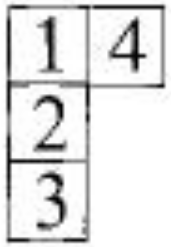
\includegraphics[scale=0.2]{build/young-21hoch2-14.png}
\begin{itemize}
\item  $\hat{A} \left(14+41
 \right) 23$ \\ 
 $= \equalInM{1234}  \equalInTableau{- 2134} \equalAntiSym{- 1324} \equalInTableau{- 3214 } \equalAntiSym{+ 2314 } \equalAntiSym{+ 3124 }
 $\\
 $ \equalInTableau{+4231} - 4132 \equalAntiSym{- 4321} - 4213 + 4123 + 4312
 $ \\
 bzw. $ abcd - bacd - acbd - cbad + cabd + bcad$\\
 $+dbca - bdca - dcba - cbda + bcda + cdba$
 \item Integrale \\
 $ + D - \frac{1}{2} \cdot (ab|ba) - 1 \cdot (bc|cb) - \frac{1}{2} \cdot (ac|ca) + 1 \cdot (ad|da) - \frac{1}{2} \cdot (bd|db) - \frac{1}{2} \cdot (cd|dc)$
\end{itemize}
\item 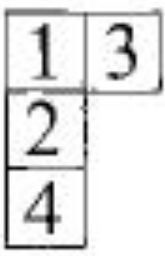
\includegraphics[scale=0.2]{build/young-21hoch2-13.png}
\begin{itemize}
\item $\hat{A} \left(13+31
 \right)24 $\\ 
 $ = \equalInM{1234} \equalInTableau{- 2134} \equalAntiSym{- 1432} \equalInTableau{- 4231} \equalAntiSym{+ 2431} \equalAntiSym{ + 4132}
 $\\
 $ \equalInTableau{+ 3214 } - 3124 \equalAntiSym{- 3412} - 3241 + 3142 + 3421
  $ \\
  bzw. $abcd - bacd - adcb - dbca + dacb + bdca$\\
  $+cbad - bcad - cdab - dbac + bdac + dcab$
  \item Integrale \\
  $+ D - 1/2 \cdot (ab|ba) - 1 \cdot (bd|db) - \frac{1}{2} \cdot (ad|da) + 1 \cdot (ac|ca) - \frac{1}{2} \cdot (bc|cb) - \frac{1}{2} \cdot (cd|dc) $
\end{itemize}
\item 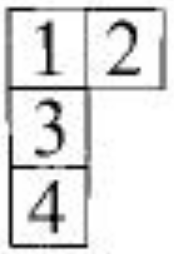
\includegraphics[scale=0.2]{build/young-21hoch2-12.png}
\begin{itemize}
\item $\hat{A} \left(12+21
 \right) 34$ \\ 
 $= \equalInM{1234} \equalInTableau{- 3214} \equalAntiSym{- 1243} \equalInTableau{- 4231} \equalAntiSym{+ 3241} \equalAntiSym{+ 4213}
 $\\
 $ \equalInTableau{+ 2134} - 2314 \equalAntiSym{- 2143} - 2431 + 2341 + 2413
 $ \\
 bzw. $abcd - cbad - abdc - dbca + dbac + cbda$\\$
+bacd - cabd - badc - dacb + dabc + cadb$
\item Integrale \\
$+ D - \frac{1}{2} \cdot (ac|ca) - 1 \cdot (cd|dc) - \frac{1}{2} \cdot (ad|da) + 1 \cdot (ab|ba) - \frac{1}{2} \cdot (bc|cb) - \frac{1}{2} \cdot (bd|db) $ 
\end{itemize}
\end{itemize}
\item $\left[ 2 ^2 \right]$ 
\begin{itemize}
\item 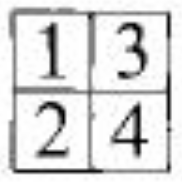
\includegraphics[scale=0.2]{build/young-2hoch2-13.png}
\begin{itemize}
\item $\hat{A} (13+31) (24+42) = \left[ \hat{A} (13+31)24  \right] - \left[ \hat{A} (13+31)42 \right]$ \\ 
$ = \equalInM{1234} \equalInTableau{- 2134} \equalInTableau{- 1243} \equalInM{+ 2143}
\equalInTableau{+ 3214} - 3124 - 4213 \equalInTableau{+ 4123} $\\
$ \equalInTableau{+ 1432} - 2431 - 1342 \equalInTableau{+ 2341}
\equalInM{+ 3412} \equalInTableau{- 3421 } \equalInTableau{- 4312 }\equalInM{+ 4321}$ \\
bzw. $ abcd - bacd - abdc + badc + cbad - bcad - cbda + bcda$\\
$+adcb - dacb - adbc + dabc + cdab - dcab - cdba + dcba$
\item Integrale \\
 $ + D -  \frac{1}{2} \cdot (ab|ba) - \frac{1}{2} \cdot (cd|dc) + 1 \cdot (ac|ca) + 1 \cdot (bd|db) - \frac{1}{2} \cdot (bc|cb) - \frac{1}{2} \cdot (ad|da)$ 
\end{itemize}
\item 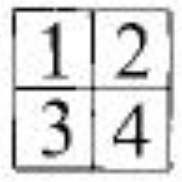
\includegraphics[scale=0.2]{build/young-2hoch2-12.png}
\begin{itemize}
\item $\hat{A} (12+21) (34+43) = \left[ \hat{A} (12+21) 34 \right] - \left[ \hat{A} (12+21)43\right]$ \\ 
$= \equalInM{1234} \equalInTableau{- 3214} \equalInTableau{- 1432} \equalInM{+ 3412}
\equalInTableau{+ 2134} - 2314 - 4132 \equalInTableau{+ 4312} $\\
$ \equalInTableau{+ 1243} - 3241 - 1423 \equalInTableau{+ 3421}
\equalInM{+ 2143} \equalInTableau{- 2341} \equalInTableau{- 4123} \equalInM{+ 4321} $  \\
bzw. 
$ abcd - cbad - adcb + cdab + bacd - cabd - bdca + cdba$\\
$+abdc - dbac - acdb + dcab + badc - dabc - bcda + dcba$
\item Integrale \\
$ + D - \frac{1}{2} \cdot (ac|ca) - \frac{1}{2} \cdot (bd|db) + 1 \cdot (ab|ba) + 1 \cdot (cd|dc) - \frac{1}{2} \cdot (bc|cb) - \frac{1}{2} \cdot (ad|da) $ 
\end{itemize}
\end{itemize}


\item  $\left[ 3\quad 1\right]$ :
\begin{itemize}
\item  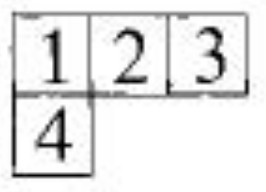
\includegraphics[scale=0.2]{build/young-31-123.png} : 
\begin{itemize}
 \item  $ \hat{A} \left( 123 +  312 + 231 + 213 + 132 +  321\right) 4$ \\
 $ = 1234 - 4231 + 3124 - 3421  + 2314 - 2341  $ \\ 
 $ + 2134 - 2431 + 1324 - 4321 + 3214 - 3241$
\end{itemize}
\item 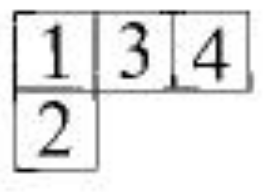
\includegraphics[scale=0.2]{build/young-31-134.png}: 
\begin{itemize}
 \item  $ \hat{A} \left( 134 + 413 + 341 + 314 + 143 + 431\right)2$ \\
 $ =1234 - 2134 + 4213 - 4123 + 3241 - 3142 $ \\
 $+ 3214 - 3124 + 1243 - 2143 + 4231 - 4132$
\end{itemize}
\item 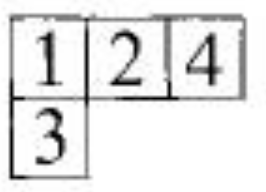
\includegraphics[scale=0.2]{build/young-31-124.png}: 
\begin{itemize}
 \item  $ \hat{A} \left( 124 + 412 + 241 + 214 + 142 + 421\right)3 $ \\
 $ =1234 - 3214 + 4132 - 4312 + 2431 - 2413 $ \\
 $ + 2134 - 2314 + 1432 - 3412 + 4231-4213 $
\end{itemize}
\end{itemize}
\item $\left[ 4\right]$ :
\begin{itemize}
\item 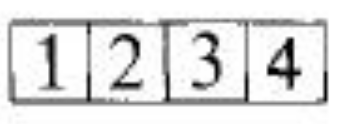
\includegraphics[scale=0.2]{build/young-4.png} : 
\begin{itemize}[label=$\ast$]
 \item \equalInM{$1234 + 1243 + 1324 + 1342 + 1423 + 1432  $\\
 $ + 2134 + 2143 + 2314 + 2341 + 2413+2431$ \\
 $ + 3124 + 3142 + 3214 + 3241 + 3412 + 3421 $\\
 $ + 4123 + 4132 + 4213 + 4231 + 4312 + 4321 $}
\end{itemize}
\end{itemize}
\end{itemize}


 
 
 \newpage
 \section{Integrale}
 \subsection{Überlappungsmatrixelemente}
 
 \subsubsection{1. Antisymmetrisieren, 2. Symmetrisieren}
 \paragraph{Spin}$ $ \\
  Überlappung gl. Tableaus $\rightarrow 1$ \\
  
  $\sigma_{12} = \sigma_{21} = \bra{\left|
  \begin{array}{c|c}
  \hline 
    1 & 3 \\ \hline 
    2 & 4 \\
    \hline 
  \end{array}
\right|_\sigma }  \ket{\left|
  \begin{array}{c|c}
  \hline 
    1 & 2 \\ \hline 
    3 & 4 \\
    \hline 
  \end{array}
 \right|_\sigma} $\\$=
 \frac{1}{\sqrt{4}} \cdot \frac{1}{\sqrt{4}}  \cdot 
 \bra{
 4\alpha\alpha\beta\beta- 4 \beta\alpha\alpha\beta- 4 \alpha\beta\beta\alpha - 4 \beta\beta\alpha\alpha
 }
 \ket{
 \beta\alpha\alpha\beta + \alpha\beta\beta\alpha- \alpha\beta\alpha\beta- \beta\alpha\beta\alpha
 }$ \\
 $ = \frac{1}{4} \cdot \left( -4 \bra{\beta\alpha\alpha\beta}\ket{\beta\alpha\alpha\beta} - 4 \bra{\alpha\beta\beta\alpha} \ket{\alpha\beta\beta\alpha}
 \right) = - 2
  $
 
 
  
 \paragraph{Ortsanteile}$ $ \\
 
 
 

 \subsubsection{1. Symmetrisieren, 2. Antisymmetrisieren}
 \paragraph{Spin}$ $ \\
 Überlappung gl. Tableaus $\rightarrow 1$ \\

(Err: 0-Wert bei Spinfunktionen) \\


 
 
 \paragraph{Ortsanteile}$ $ \\


 
 \subsection{Hamiltonmatrixelemente}
 \subsubsection{1. Antisymmetrisieren, 2. Symmetrisieren}
  \paragraph{Spin}$ $ \\
  s. Überlappung
 \paragraph{Ortsanteile}$ $ \\
 \subsubsection{1. Symmetrisieren, 2. Antisymmetrisieren }
  \paragraph{Spin}$ $ \\
  s. Überlappung
 \paragraph{Ortsanteile}$ $ \\
  \begin{gather}
\Phi_{11} = \bra{
\left|
  \begin{array}{c|c}
  \hline 
    1 & 2 \\ \hline 
    3 & 4 \\
    \hline 
  \end{array}
\right| _{\Phi}
} \hat{H} \ket{
\left|
  \begin{array}{c|c}
  \hline 
    1 & 2 \\ \hline 
    3 & 4 \\
    \hline 
  \end{array}
\right| _{\Phi}
} \\
 = + D - \frac{1}{2} \cdot (ac|ca) - \frac{1}{2} \cdot (bd|db) + 1 \cdot (ab|ba) + 1 \cdot (cd|dc) - \frac{1}{2} \cdot (bc|cb) - \frac{1}{2} \cdot (ad|da) 
 \end{gather} \\


\begin{gather}
\Phi_{12} = \bra{
\left|
  \begin{array}{c|c}
  \hline 
    1 & 2 \\ \hline 
    3 & 4 \\
    \hline 
  \end{array}
\right| _{\Phi}
} \hat{H} \ket{
\left|
  \begin{array}{c|c}
  \hline 
    1 & 3 \\ \hline 
    2 & 4 \\
    \hline 
  \end{array}
\right| _{\Phi}
} \\
 = - \frac{1}{4} \cdot D - \frac{1}{4} \cdot (ab|ba) - \frac{1}{4} \cdot (cd|dc) - \frac{1}{4} \cdot (ac|ca) -  \frac{1}{4} \cdot (bd|db) + \frac{1}{2} \cdot (bc|cb) + \frac{1}{2} \cdot (ad|da) 
 \end{gather} \\



\begin{gather}
\Phi_{22} = \bra{
\left|
  \begin{array}{c|c}
  \hline 
    1 & 3 \\ \hline 
    2 & 4 \\
    \hline 
  \end{array}
\right| _{\Phi}
} \hat{H} \ket{
\left|
  \begin{array}{c|c}
  \hline 
    1 & 3 \\ \hline 
    2 & 4 \\
    \hline 
  \end{array}
\right| _{\Phi}
} \\
= + D -  \frac{1}{2} \cdot (ab|ba) - \frac{1}{2} \cdot (cd|dc) + 1 \cdot (ac|ca) + 1 \cdot (bd|db) - \frac{1}{2} \cdot (bc|cb) - \frac{1}{2} \cdot (ad|da)
\end{gather} \\

























\end{document}